\documentclass[11pt]{article}
\usepackage[a4paper,margin=1.9cm]{geometry}
\usepackage[T1]{fontenc}
\usepackage{textcomp}
\usepackage{amsmath,amssymb}
\usepackage{enumitem}
\usepackage{tikz}
\usetikzlibrary{calc,arrows.meta,patterns,decorations.pathmorphing}
\usepackage{xcolor}
\usepackage{multicol}
\usepackage{parskip}
\usepackage{lmodern}
\renewcommand{\familydefault}{\sfdefault}

\definecolor{unalblue}{RGB}{31,73,124}

\newlist{opciones}{enumerate}{1}
\setlist[opciones]{label=(\alph*),itemsep=1pt,topsep=2pt,leftmargin=1.8em,font=\normalfont}

\newcommand{\vect}[2]{\begin{pmatrix}#1\\#2\end{pmatrix}}
\newcommand{\vectiii}[3]{\begin{pmatrix}#1\\#2\\#3\end{pmatrix}}

\newcommand{\examheader}{%
  \noindent
  \begin{minipage}[t]{0.62\linewidth}
    {\bfseries\large Universidad Nacional de Colombia, sede Medell\'in}\\
    {\small Facultad de Ciencias --- Escuela de Matem\'aticas}\\
    {\small Primer Examen Parcial de C\'alculo en Varias Variables}\\
    {\small 14 de marzo de 2015}
  \end{minipage}%
  \hfill
  \begin{minipage}[t]{0.33\linewidth}
    \raggedleft\small
    Nombre: \rule{3cm}{0.4pt}\\[4pt]
    Doc. identidad: \rule{2.5cm}{0.4pt}
  \end{minipage}\\[4pt]
  \rule{\linewidth}{0.6pt}
}
\newcommand{\examfooter}{%
  \vfill
  \rule{\linewidth}{0.4pt}\\[1pt]
  {\scriptsize\textit{Transcripci\'on digital --- MathUNAL}\hfill\textcolor{unalblue}{\textbf{\thepage}}}
}
\pagestyle{empty}

\begin{document}

\examheader

\textbf{Instrucciones.} El examen tiene una duraci\'on de 1 hora y 40 minutos. No se admiten preguntas durante el examen. No est\'a permitido el uso de calculadora, ni tel\'efonos m\'oviles, ni cualquier otro tipo de aparato electr\'onico. Los tel\'efonos m\'oviles deben estar guardados. Cualquier intento de fraude ser\'a sancionado con anulaci\'on del examen. En los puntos 2., 3. y 4. justifique sus respuestas.

\bigskip

\textbf{1.} En los siguientes numerales no necesita justificar su respuesta. Elija solo la opci\'on correcta en cada caso.

\medskip
\textit{a)} (8\,\%) Considere las gr\'aficas de las siguientes superficies

\begin{center}
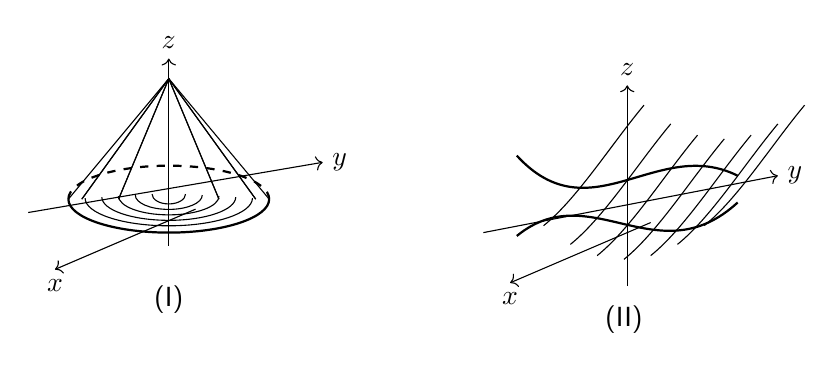
\begin{tikzpicture}[scale=0.85]
  % Superficie (I): paraboloide hacia abajo z = 1 - x^2 - y^2, malla tipo domo
  \begin{scope}
    % malla de meridianos
    \foreach \a in {0,30,...,150}{
      \draw[thin] ({1.5*cos(\a)},{0.0}) -- (0,1.8) -- ({-1.5*cos(\a)},{0.0});
    }
    \foreach \t in {0.3,0.6,0.9,1.2,1.5,1.8}{
      \draw[thin] ({-1.5*(1-\t/1.8)},{\t*0.05}) arc (180:360:{1.5*(1-\t/1.8)} and {0.4*(1-\t/1.8)+0.08});
    }
    \draw[thick] (-1.5,0) arc (180:360:1.5 and 0.5);
    \draw[thick,dashed] (-1.5,0) arc (180:0:1.5 and 0.5);
    \draw[->] (0,-0.7) -- (0,2.1) node[above]{$z$};
    \draw[->] (-2.1,-0.2) -- (2.3,0.55) node[right]{$y$};
    \draw[->] (0.4,-0.15) -- (-1.7,-1.05) node[below]{$x$};
    \node at (0,-1.5) {(I)};
  \end{scope}
  % Superficie (II): silla de montar hiperbólica z = x^2 - y^2
  \begin{scope}[xshift=6.8cm]
    \foreach \s in {-1.2,-0.8,-0.4,0,0.4,0.8,1.2}{
      \draw[thin] ({\s},{0.35*\s*\s-0.9}) .. controls ({\s+0.5},{0.35*\s*\s-0.5}) and ({\s+1.0},{0.35*\s*\s+0.3}) .. ({\s+1.5},{0.35*\s*\s+0.9});
    }
    \draw[thick] (-1.6,-0.55) .. controls (-0.5,0.35) and (0.5,-1.15) .. (1.7,-0.05);
    \draw[thick] (-1.6,0.65) .. controls (-0.5,-0.55) and (0.5,0.95) .. (1.7,0.35);
    \draw[->] (0.05,-1.3) -- (0.05,1.7) node[above]{$z$};
    \draw[->] (-2.1,-0.5) -- (2.3,0.35) node[right]{$y$};
    \draw[->] (0.4,-0.35) -- (-1.7,-1.25) node[below]{$x$};
    \node at (0,-1.8) {(II)};
  \end{scope}
\end{tikzpicture}
\end{center}

Podemos afirmar
\begin{opciones}
  \item Una ecuaci\'on para (I) es $z = 1-x^2-y^2$, mientras que una ecuaci\'on para (II) es $z=\sin(x)\cos(y)$.
  \item Una ecuaci\'on para (I) es $z = x^2-y^2$, mientras que una ecuaci\'on para (II) es $z^2=x^2+2y^2$.
  \item Una ecuaci\'on para (I) es $z = 1-x^2-y^2$, mientras que una ecuaci\'on para (II) es $z=\dfrac{xy}{x^2+y^2}$.
  \item Una ecuaci\'on para (I) es $z = x^2-y^2$, mientras que una ecuaci\'on para (II) es $z=\dfrac{xy}{x^2+y^2}$.
\end{opciones}

\medskip
\textit{b)} (8\,\%) Si $f$ es una funci\'on diferenciable en todo $\mathbb{R}^2$ y el plano tangente a la gr\'afica de $f$ en el punto $(1,1)$ es $z=5x+2y+7$, entonces

\begin{opciones}
  \item $f(1,1)=7$.
  \item $f_x(1,1)=2$.
  \item $f_y(1,1)=2$.
  \item Ninguna de las anteriores.
\end{opciones}

\medskip
\textit{c)} (8\,\%) Considere las siguientes afirmaciones

\medskip
A. Si $f(x,y)$ es diferenciable en $(0,0)$ entonces $f_{xy}(0,0)=f_{yx}(0,0)$.

B. Si $f_x(0,0)=f_y(0,0)$ entonces $f(x,y)$ es diferenciable en $(0,0)$.

\medskip
Podemos afirmar:
\begin{opciones}
  \item Solo A es verdadera.
  \item Solo B es verdadera.
  \item Tanto A como B son verdaderas.
  \item Tanto A como B son falsas.
\end{opciones}

\medskip
\textit{d)} (8\,\%) Si $f$ es una funci\'on de clase $C^1$ cuyas derivadas parciales de segundo orden existen, entonces puede asegurarse que:

\begin{opciones}
  \item $f_x$ y $f_y$ son funciones diferenciables.
  \item Las derivadas cruzadas $f_{xy}$ y $f_{yx}$ son las mismas.
  \item $f_{xx}$ y $f_{yy}$ son funciones continuas.
  \item Ninguna de las anteriores.
\end{opciones}

\medskip
\textit{e)} (8\,\%) La funci\'on $f$ cuyas curvas de nivel corresponden a las mostradas en la siguiente figura, es

\begin{center}
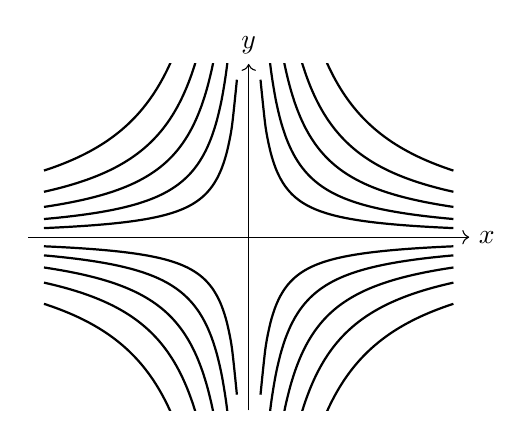
\begin{tikzpicture}[scale=1.0]
  \begin{scope}
    \clip (-2.8,-2.2) rectangle (2.8,2.2);
    \path[use as bounding box] (-2.8,-2.2) rectangle (2.8,2.2);
    % Familia de hiperbolas xy = c, c>0 en cuadrantes I y III, c<0 en II y IV
    \foreach \c in {0.3,0.6,1.0,1.5,2.2}{
      \draw[thick,domain=0.15:2.6,samples=40,smooth,variable=\x] plot ({\x},{\c/\x});
      \draw[thick,domain=-2.6:-0.15,samples=40,smooth,variable=\x] plot ({\x},{\c/\x});
      \draw[thick,domain=0.15:2.6,samples=40,smooth,variable=\x] plot ({\x},{-\c/\x});
      \draw[thick,domain=-2.6:-0.15,samples=40,smooth,variable=\x] plot ({\x},{-\c/\x});
    }
  \end{scope}
  \draw[->] (-2.8,0) -- (2.8,0) node[right]{$x$};
  \draw[->] (0,-2.2) -- (0,2.2) node[above]{$y$};
\end{tikzpicture}
\end{center}

\begin{opciones}
  \item $f(x,y)=\dfrac{1}{x^2+y^2+1}$.
  \item $f(x,y)=x^2+y^2$.
  \item $f(x,y)=xy$.
  \item Ninguna de las anteriores.
\end{opciones}

\newpage
\examheader
\vspace{2pt}

\textbf{2.} (15\,\%) Hallar los puntos sobre el hiperboloide de una hoja $-x^2+z^2+y^2=1$ donde el plano tangente a \'el es paralelo al plano $z=4y-5$.

\bigskip
\bigskip

\textbf{3.} Sea $f:\mathbb{R}^2\to\mathbb{R}$ la funci\'on definida por
$$
f(x,y)=
\begin{cases}
\dfrac{x^4+y^4}{x^2+y^2}+x-2y, & (x,y)\neq (0,0)\\[4pt]
0, & (x,y)=(0,0)
\end{cases}
$$

\begin{opciones}
  \item[i.] (8\,\%) Encuentre $f_x(0,0)$ y $f_y(0,0)$.
  \item[ii.] (12\,\%) Muestre que $f$ es diferenciable en $(0,0)$.
  \item[iii.] (5\,\%) Encuentre la derivada direccional de $f$ en el punto $(0,0)$ en la direcci\'on del vector $v=(-3,4)$.
\end{opciones}

\vfill
\examfooter
\newpage
\examheader
\vspace{2pt}

\textbf{4.} Sea $f:\mathbb{R}^2\to\mathbb{R}$ una funci\'on de clase $C^2$ de la cual se tiene la siguiente informaci\'on:
\begin{itemize}[itemsep=1pt,topsep=2pt]
  \item $\nabla f(1,1)=(2,-3)$.
  \item $\nabla f(1,0)=(5,-2)$.
  \item $f_{xx}(1,1)=f_{yy}(1,1)=f_{xy}(1,1)=10$.
  \item $f_{xx}(1,0)=f_{yy}(1,0)=f_{xy}(1,0)=-8$.
\end{itemize}

Definamos $g(u,v)=f(2-u^2v,\,uv-1)$.

\begin{opciones}
  \item[a)] (6\,\%) Encuentre una expresi\'on para $g_u(u,v)$.
  \item[b)] (14\,\%) Hallar $g_{uv}(1,1)$.
\end{opciones}

\vfill
\examfooter

\end{document}
